\documentclass[10pt,twocolumn]{article}

% use the oxycomps style file
\usepackage{oxycomps}

% usage: \fixme[comments describing issue]{text to be fixed}
% define \fixme as not doing anything special
\newcommand{\fixme}[2][]{#2}
% overwrite it so it shows up as red
\renewcommand{\fixme}[2][]{\textcolor{red}{#2}}
% overwrite it again so related text shows as footnotes
%\renewcommand{\fixme}[2][]{\textcolor{red}{#2\footnote{#1}}}

% read references.bib for the bibtex data
\bibliography{references}

% include metadata in the generated pdf file
\pdfinfo{
    /Title (The Occidental Computer Science Comprehensive Project: Goals, Timeline, Format, and Advice)
    /Author (Bernie Cassidy)
}

% set the title and author information
\title{Generating Musical Sequences with Recurrent Neural Networks: \\ A TensorFlow Tutorial}
\author{Bernie Cassidy}
\affiliation{Occidental College}
\email{bcassidy@oxy.edu}

\begin{document}

\maketitle

\section{Introduction}

For my comps project, I am planning to design digital instruments using the Max/MSP visual programming language, use neural networks to create musical sequences generated by artificial intelligence, and combine the two processes to make a final product of hybrid human- and AI-made musical compositions.

In order to begin making artificially-generated music, I went through the tutorial "Generate music with an RNN", which uses TensorFlow to generate sequences of music notes using a recurrent neural network (RNN). The network is trained to predict the next note in a musical sequence using a "collection of piano MIDI files from the MAESTRO dataset". \cite{TensorFlow2021GenerateMusic} The goal of this tutorial is to generate a string of musical notes, represented in MIDI files, that sound similar to the sequences in the MAESTRO dataset.

Ideally, these musical sequences would be both interesting (not overly repetitive or simplistic) and cohesive (notes flow together and don't sound like they were randomly generated). While the process in the tutorial was straightforward, I found it hard to achieve both of these qualities, and pursuing artificially-generated music that is cohesive and interesting will likely be a focus of a lot of the work done in my comps project.


\section{Methods}

The tutorial uses the MAESTRO dataset \cite{hawthorne2018enabling}, which consists of recordings of piano performances captured and converted to MIDI data; the pretty\_midi library\cite{prettyMIDI}, a Python library created to handle MIDI data; and the pyFluidSynth module \cite{pyFluidSynth}, which allows the FluidSynth software synthesizer to be used in Python programs. It also uses the numpy, pandas, seaborn and tensorflow Python libraries. I went through the tutorial using Google Colab, and started by downloading and setting up the aforementioned libraries, packages, and datasets. PyFluidSynth was not necessary for generating musical sequences, but it was included in the tutorial to allow the user to play sequences from the dataset and music generated during the tutorial out loud in Colab. 


\subsection{Introduction to MIDI}

For the next section, I processed and inspected a MIDI file using the pretty\_midi library, downloading a sample file from the MAESTRO dataset, generating a pretty\_midi object for that file, and then analyzing the instruments used in the audio sample before listening to the sample. Following the tutorial, I then extracted each individual note from the sample file and generated a table, reproduced in Figure \ref{fig:table}, displayed each note's data, including its pitch, duration, and distance from the previous note. In this table the pitches are represented by MIDI values, but the tutorial also gave me the option to display them using their note names (e.g. C3 or D4). Next it let me generate a visualization of the entire audio file in piano roll format, and plot the distribution of each note variable (see Figure \ref{fig:distributions}).

\begin{figure}
    \centering
    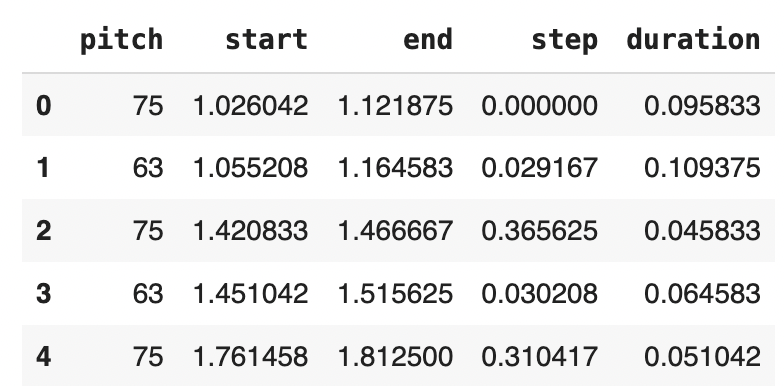
\includegraphics[width=0.75\linewidth]{Table.png}
    \caption{Table of first notes in sample file}
    \label{fig:table}
\end{figure}

Now that I was familiar with the pretty\_midi library, it was time to generate my own MIDI file, reverse-engineering the sample audio file from the list of notes that I had just generated. The tutorial did this using a function that iterates over each note in the list's data and converts them to pretty\_midi note objects. When I played the file generated by this process, it was indistinguishable from the sample audio file I had downloaded.

\begin{figure}
    \centering
    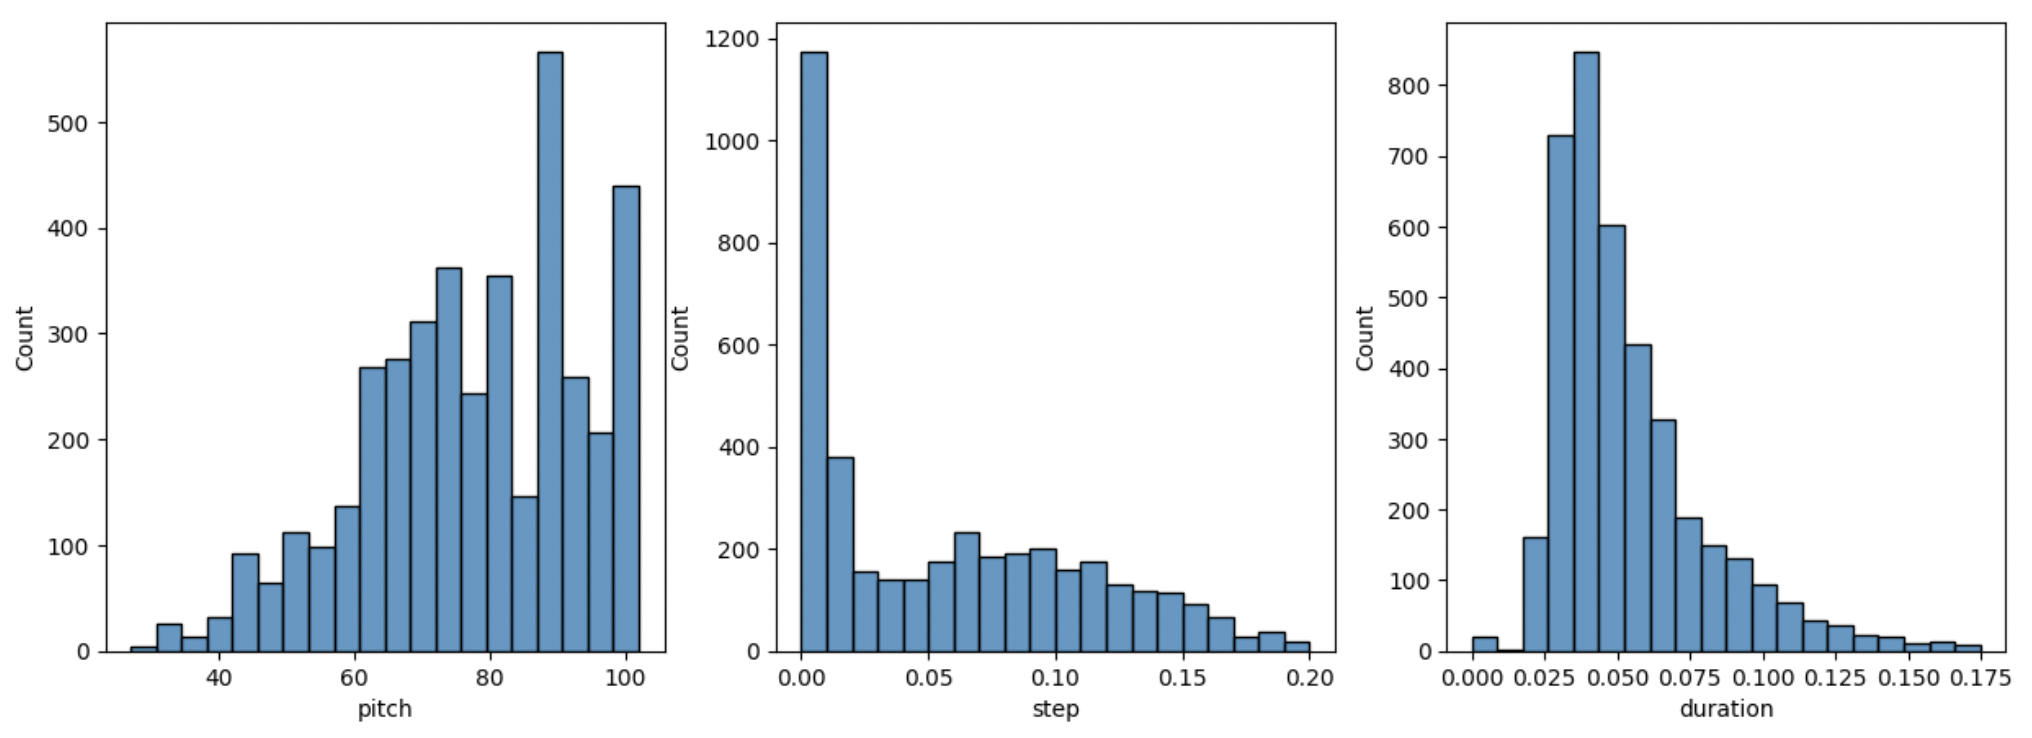
\includegraphics[width=1\linewidth]{Distributions.png}
    \caption{Distributions of note variables from sample file}
    \label{fig:distributions}
\end{figure}

\subsection{Training the Model}

Now it was time to create the training dataset by extracting note sequences from the MAESTRO dataset's MIDI files. I chose to use 50 of MAESTRO's over 1200 files to create the dataset, which amounted to over 215,000 notes, and made a TensorFlow Dataset using these notes and their pitch, duration and step values. Using this dataset, I created 50-note sequences to train the neural network. 

The model would have three outputs (representing pitch, duration and step), with custom loss functions for each output. Since more variability would be expected from the pitch variable, the loss from that output was weighted twenty times less than the loss for duration and step when creating a single loss function to measure the model. It would take in note sequences and then output the note it predicted to be next in the sequence, then measure the difference between the predicted note and the actual next note. The model was then set to be trained over fifty epochs, but after eighteen epochs and nearly nine minutes, the process was stopped early. The model's loss decreased steadily over training periods, but it increased dramatically and fluctuated over the last several epochs (see Figure \ref{fig:loss} for a graph of loss per epoch).

\begin{figure}
    \centering
    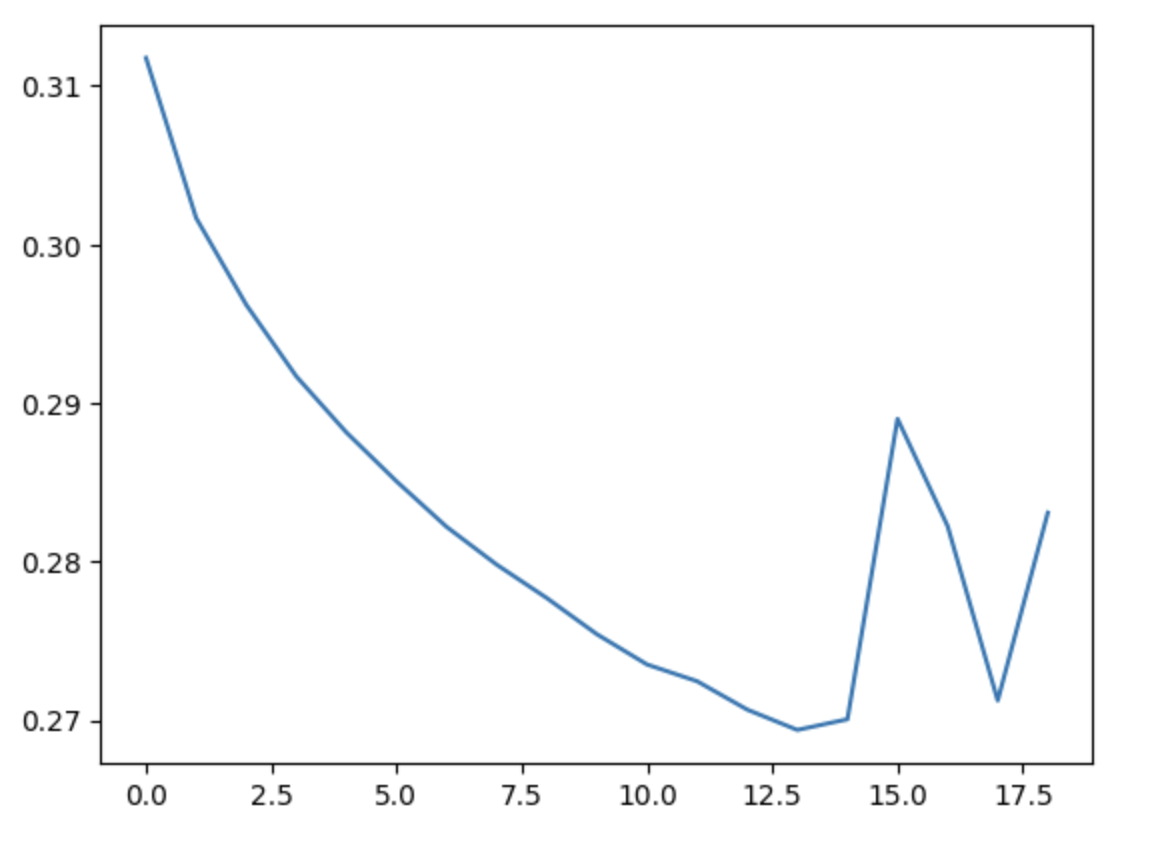
\includegraphics[width=0.75\linewidth]{Loss.png}
    \caption{Loss for each training epoch}
    \label{fig:loss}
\end{figure}


\subsection{Generating Musical Sequences}

Now it was finally time to generate my own sequence of notes. Using the note-prediction function, the model took a sample note sequence, appended its prediction to the sequence, and then predicted the next note for the updated sequence after each new prediction. I was able to play around with the temperature (which determined randomness of each prediction) and the length of each predicted sequence. The model generated a thirty-second long sequence that I was able to listen to, but I was somewhat disappointed with the results. The sequence was very repetitive at the temperature the tutorial started with, but increasing the temperature just made the new sequences sound random and off-key. The following section will discuss these results in further detail.


\section{Metrics and Results}

Measuring how well the model performs in generating musical sequences was never going to be easy, because music is difficult to quantify and open to each listener's interpretation. In the first section of the paper, I introduced two qualitative criteria that I was seeking from the model's musical sequences: I wanted them to be both interesting and cohesive. In terms of the three outputs the model generates for each note, I would say that this means I am seeking distributions for pitch, step, and duration that are neither completely uniform nor concentrated on only a few values. I think that finding more specific ranges for these distributions will be an important next step in my comps project, and it will take lots of trial and error to find the ranges that I like listening to the most.

That being said, the tutorial included the distributions of note variables from the musical sequence that the model generated, which can be found in Figure \ref{fig:generated-dist}. When comparing it to the distributions from the sample file (Figure \ref{fig:distributions}), it is clear that while there is variation in pitch, the step and duration values do not vary much at all from note to note. Increasing the "temperature" of the generation function barely altered the distribution of step and duration values, so fixing this lack of diversity in step and duration of notes will not be easy.

\begin{figure}
    \centering
    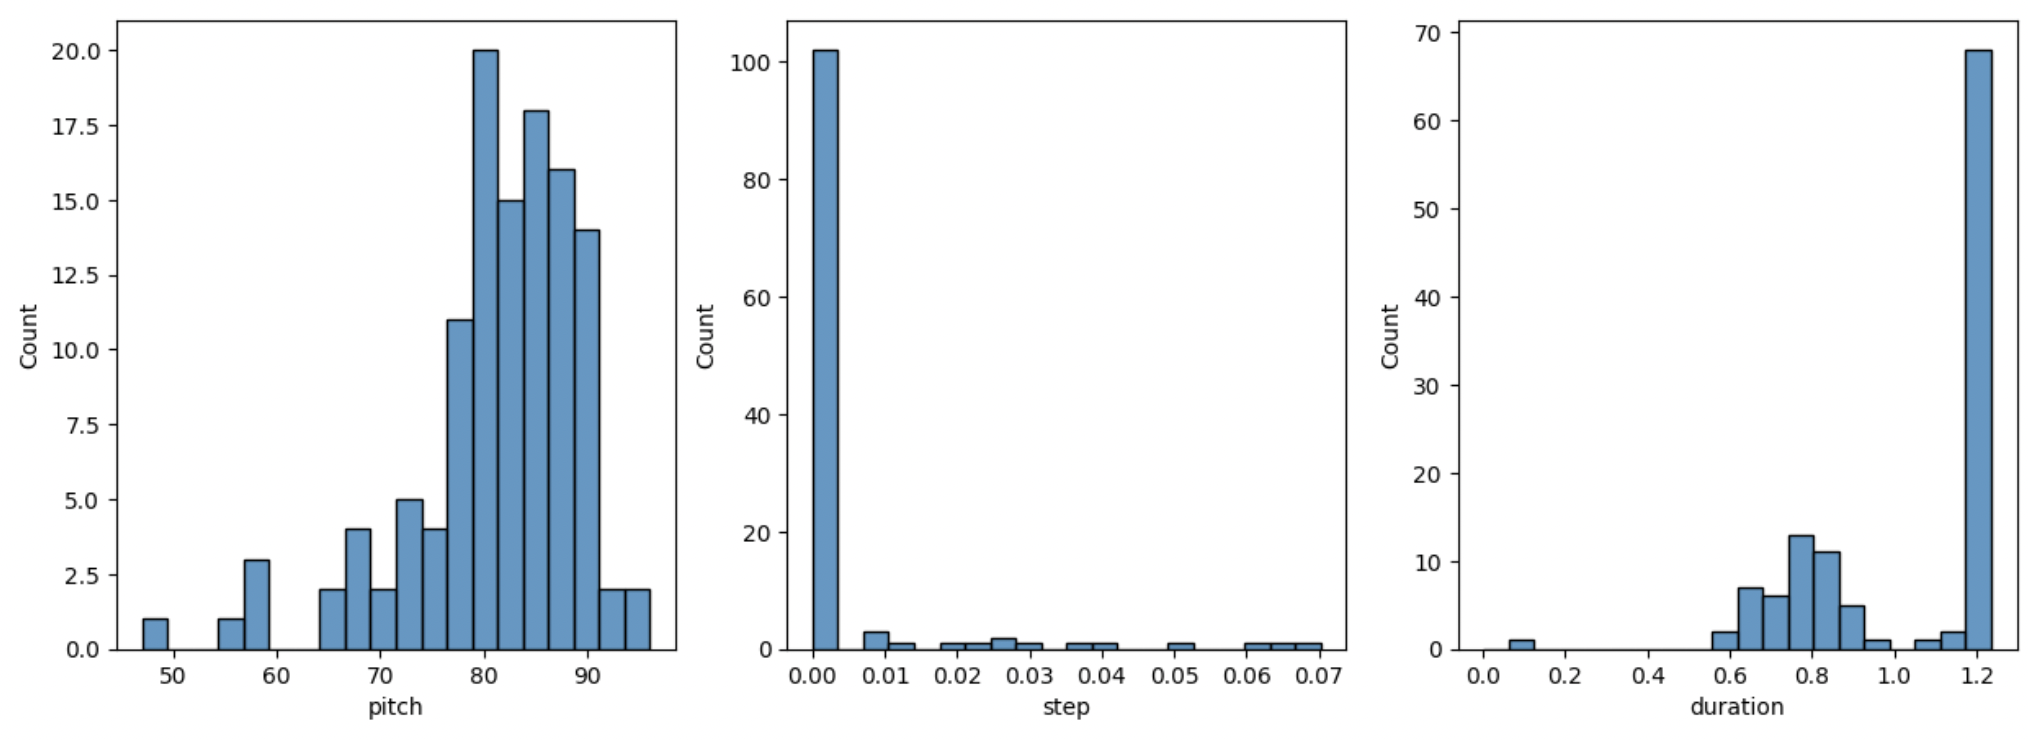
\includegraphics[width=1\linewidth]{GeneratedDist.png}
    \caption{Distributions of note variables from generated sequence}
    \label{fig:generated-dist}
\end{figure}

The tutorial was successful in teaching me how to generate musical sequences using neural networks and in giving me a way to measure how well these sequences fit my criteria of both interesting and cohesive music. However, actually training a model to create musical sequences that are interesting and cohesive will be a much more difficult task.


\section{Reflection}

I would say that this tutorial helped me start on the road to achieving what I want to accomplish with my comps process, but also showed me that there is a long way to go. I have definitely learned more about generating music using artificial intelligence, and about training neural networks in general. I enjoyed the process a lot and it made me excited to work on this topic for my comps project, but I am concerned because I have to learn a lot more and figure both what exactly I am looking for from a model and how to fine-tune a model to achieve that goal.

\printbibliography


\end{document}